\documentclass[tikz,border=6pt]{standalone}
\usepackage{tikz}
\usetikzlibrary{arrows.meta}
\begin{document}
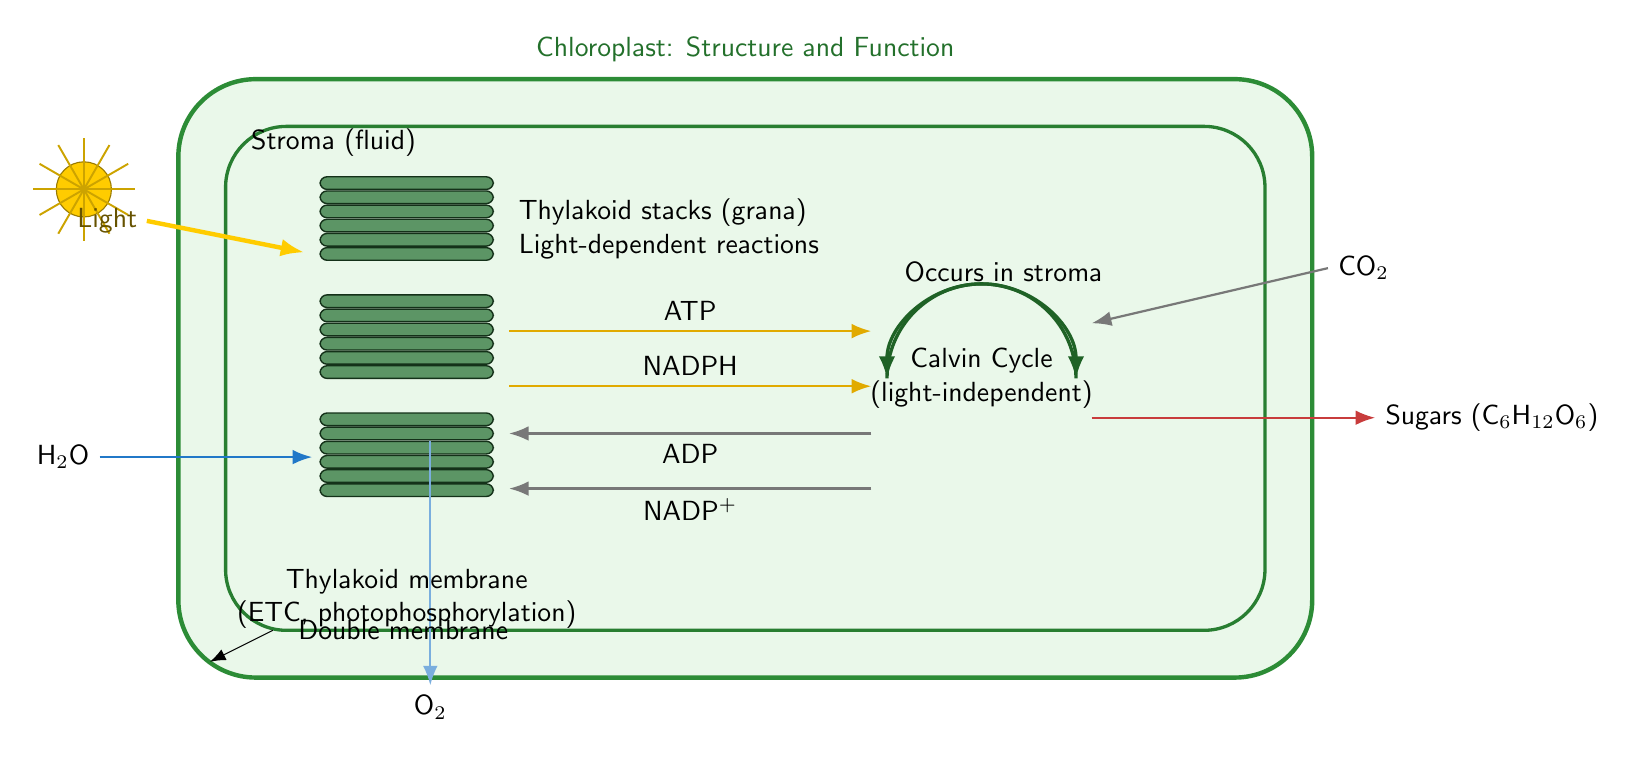
\begin{tikzpicture}[font=\sffamily]
% Colors
\definecolor{chloro}{RGB}{44,140,54}
\definecolor{thyla}{RGB}{51,122,62}
\definecolor{stroma}{RGB}{234,248,234}
\definecolor{light}{RGB}{255,204,0}
\definecolor{sugar}{RGB}{200,60,60}
\definecolor{water}{RGB}{33,120,200}
\definecolor{energy}{RGB}{225,170,0}
\definecolor{return}{RGB}{120,120,120}

% Chloroplast stroma background
\path[fill=stroma, rounded corners=28pt] (-7.2,-3.8) rectangle (7.2,3.8);
% Double membrane outlines
\draw[line width=1.6pt, chloro, rounded corners=28pt] (-7.2,-3.8) rectangle (7.2,3.8);
\draw[line width=1.2pt, chloro!90!black, rounded corners=22pt] (-6.6,-3.2) rectangle (6.6,3.2);

% Title
\node[anchor=south, text=chloro!80!black] at (0,3.9) {Chloroplast: Structure and Function};

% Stroma label
\node[anchor=west, text=black] at (-6.4,3.0) {Stroma (fluid)};

% Thylakoid stacks (grana)
\foreach \y in {-1.5,0,1.5}{
  \foreach \k in {0,...,5}{
    \path[fill=thyla!80, draw=thyla!40!black, line width=0.5pt, rounded corners=2.5pt]
      (-5.4, \y + 0.18*\k) rectangle (-3.2, \y + 0.18*\k + 0.16);
  }
}
\node[anchor=west, align=left] at (-3.0,1.9) {Thylakoid stacks (grana)\\Light-dependent reactions};

% Light hitting thylakoids (sun + ray + arrow)
\draw[fill=light, draw=light!60!black] (-8.4,2.4) circle (0.35);
\foreach \a in {0,30,...,330}{
  \draw[light!80!black, line width=0.7pt] (-8.4,2.4) -- ++(\a:0.65);
}
\draw[-{Latex[length=3mm]}, ultra thick, light] (-7.6,2.0) -- (-5.6,1.6);
\node[anchor=east, text=light!40!black] at (-7.6,2.0) {Light};

% Water in, Oxygen out
\draw[-{Latex[length=2.5mm]}, thick, water] (-8.2,-1.0) node[left, black]{H$_2$O} -- (-5.5,-1.0);
\draw[-{Latex[length=2.5mm]}, thick, water!60] (-4.0,-0.8) -- (-4.0, -3.9) node[below, black]{O$_2$};

% Calvin Cycle on the stroma side (circular arrows)
\draw[-{Latex[length=2.8mm]}, line width=1.2pt, chloro!70!black] (1.8,0) arc[start angle=180, end angle=0, radius=1.2];
\draw[-{Latex[length=2.8mm]}, line width=1.2pt, chloro!70!black] (4.2,0) arc[start angle=0, end angle=180, radius=1.2];
\node[align=center] at (3,0) {Calvin Cycle\\(light-independent)};

% Energy carriers between thylakoids and Calvin cycle
\draw[-{Latex[length=2.5mm]}, thick, energy] (-3.0,0.6) -- (1.6,0.6) node[midway, above, black]{ATP};
\draw[-{Latex[length=2.5mm]}, thick, energy] (-3.0,-0.1) -- (1.6,-0.1) node[midway, above, black]{NADPH};

\draw[-{Latex[length=2.5mm]}, thick, return] (1.6,-0.7) -- (-3.0,-0.7) node[midway, below, black]{ADP};
\draw[-{Latex[length=2.5mm]}, thick, return] (1.6,-1.4) -- (-3.0,-1.4) node[midway, below, black]{NADP$^+$};

% CO2 in to Calvin cycle
\draw[-{Latex[length=2.5mm]}, thick, return] (7.4,1.4) node[right, black]{CO$_2$} -- (4.4,0.7);

% Sugar out
\draw[-{Latex[length=2.5mm]}, thick, sugar] (4.4,-0.5) -- (8.0,-0.5) node[right, black]{Sugars (C$_6$H$_{12}$O$_6$)};

% Compartment labels
\node[anchor=north, align=center, text=black] at (-4.3,-2.3) {Thylakoid membrane\\(ETC, photophosphorylation)};
\node[anchor=north west, text=black] at (1.9,1.6) {Occurs in stroma};

% Double membrane note
\draw[-{Latex[length=2mm]}, thin] (-6.0,-3.2) -- (-6.8,-3.6);
\node[anchor=west, align=left] at (-5.8,-3.2) {Double membrane};

\end{tikzpicture}
\end{document}
